
\chapter{Preliminary results}

{\hypersetup{linkcolor=GREYDARK}\minilof\newpage}

\graphicspath{{chap7-Translational Selection/figures/}}


\begin{figure}[t]
    \centering                                                                            
    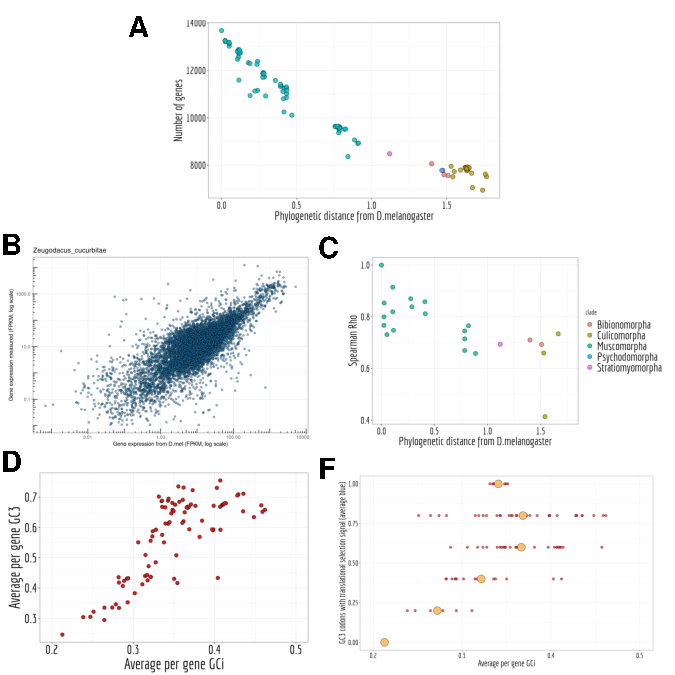
\includegraphics[width=\textwidth] {figures/Appen_C1.pdf}                                               
    \caption[Translational selection in Diptera]{\textbf{Translational selection in Diptera.} \textbf{A}: Number of genes with reciprocal blast hits with \textit{D. melanogaster} for 95 dipterans, and phylogenetic distance from \textit{D. melanogaster}. \textbf{B}: Gene expression measured in \textit{Z. cucurbitae} compared to the gene expression measured in \textit{D. melanogaster} for genes with reciprocal blast hits. \textbf{C}: Spearmann coefficient (rho), corresponding to the graphic in \textbf{B}, for 22 species for which gene expression data were available. X-axis is the phylogenetic distance from \textit{D. melanogaster}. \textbf{D}: Relationship between GC3 and GCi for the 95 dipterans studied. \textbf{F}: Relationship between the GC3 of codons optimizing translation and GCi for the 95 dipterans studied.}
    \label{suppfig:AppC1}
\end{figure}


\begin{figure}[t]
    \centering                                                                            
    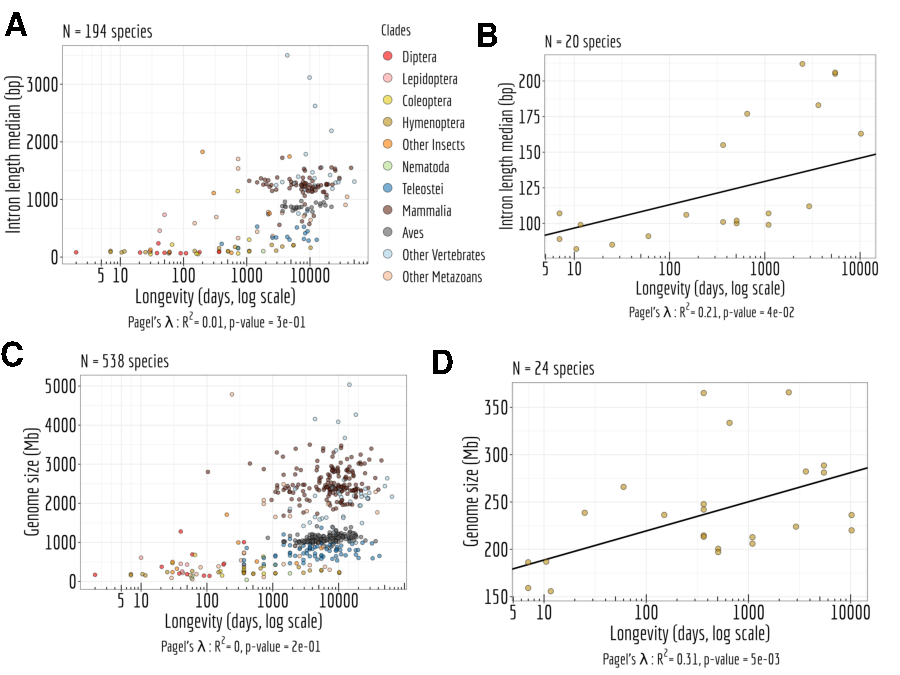
\includegraphics[width=\textwidth] {figures/Appen_C2.pdf}                                   
     \caption[Impact of \Ne~on introns length and genomes size]{\textbf{Impact of \Ne~on introns length and genomes size.} \textbf{A}: Relationship between median intron length and longevity (days, log scale) per species from GTDrift. \textbf{B}: Relationship between median intron length and longevity (days, log scale) focused on hymenopterans. \textbf{C}: Relationship between genomes size (Mb) and longevity (days, log scale). \textbf{D}: Relationship between genomes size (Mb) and longevity (days, log scale) focused on hymenopterans. 
     Pagel's \textit{lambda} model is used to take into account the phylogenetic structure of the data in a regression model (black line if significant).} 
    \label{suppfig:AppC2}
\end{figure}